\author{Andrei Tkachuk}

\section{Экстремум функции нескольких переменных}

    \begin{Def}[Экстремума ФНП]
		Пусть функция $u = f(M) = f(x_1, \dots, x_n)$ --- является функцией n - переменных определённых в некоторой окрестности $U(M_0)$ и $M_0(x^0_1, \dots, x^0_n)$.\\
		Тогда
		\begin{enumerate}
			\item $M_0$ --- точкой (локального) минимума функции $f(M)$, если \\ 
            $\exists \delta > 0, \, \forall M \in U_\delta(M_0), \, f(M) \geqslant f(M_0)$
			
            \item $M_0$ --- точкой (локального) максимума функции $f(M)$, если \\ 
            $\exists \delta > 0, \, \forall M \in U_\delta(M_0), \, f(M) \leqslant f(M_0)$
            
        	\item $M_0$ --- точкой (локального) экстремума $f(M)$, если \\
             $M_0 = \min f(M)$ или $M_0 = \max f(M)$
		\end{enumerate}
	\end{Def}
	\begin{Def}[Строгий экстремум функции нескольких переменных]
		Пусть функция $u = f(M) = f(x_1, \dots, x_n)$ --- является функцией n - переменных определённых в некоторой окрестности $U(M_0)$ и $M_0(x^0_1, \dots, x^0_n)$\\
		Тогда
		\begin{enumerate}
			\item $M_0$ --- точкой строгого минимума функции $f(M)$, если\\
            $\exists \delta > 0, \, \forall M \in \mathring{U}(M_0), \, f(M) > f(M_0)$
            
			\item $M_0$ --- точкой строгого максимума функции $f(M)$, если\\
            $\exists \delta > 0, \, \forall M \in \mathring{U}(M_0), \, f(M) < f(M_0)$
			
            \item $M_0$ --- точкой строгого экстремума функции $f(M)$, если соблюдается пункт 1 или 2
		\end{enumerate}	
	\end{Def}

	\begin{Th}[Необходимое условие локального экстремума]
		Пусть существует функция 
        \begin{align*}
            &u = f(M) = f(x_1, \dots, x_n), \, M \in U_0(M_0)\\
            &\text{где }  M_0(x^0_1, \dots, x^0_n) \, \text{и } \exists f'_{x_1}, \dots, f'_{x_n}
        \end{align*}
		Тогда если $M_0$ --- точка локального экстремума, то 
        \[
            f'_{x_1}(M_0) = 0, \dots, f'_{x_n}(M_0) = 0 \Leftrightarrow df(M_0) = 0
        \]
	\end{Th}
	\begin{Proof}
		Пусть $M_0$ --- минимум f(M), т.е. 
        \[
            \exists \delta > 0, \, \forall M \in U_\delta(M_0), \, f(M) \geqslant f(M_0)
        \]
		Рассмотрим частную производную от первого аргумента через предел. Для этого возьмём точку $M(x_1, x^0_2, \dots, x^0_n)$ в окрестности точки $M_0$, тогда получаем\\
		\[
            f'_{x_1}(M_0) = \lim_{x_1 \to x^0_1}(\frac{f(x_1, x^0_2, \dots, x^0_n) - f(x^0_1, \dots, x^0_n)}{x_1 - x^0_1})
        \]
		Так как $M_0$ ---  минимум $f(M)$, то 
        \[
            f(M) - f(M_0) \geqslant 0
        \]
		Осталось рассмотреть два случая для знаменателя
		\begin{enumerate}
			\item если $x_1 > x^0_1$, то $f'_{x_1} \geqslant 0$
			\item если $x_1 < x^0_1$, то $f'_{x_1} \leqslant 0$
		\end{enumerate}
		Из всего этого следует, что 
        \[
            f'_{x_1}(M_0) = 0
        \] 
		Аналогично доказываются случаи для других производных
	\end{Proof}

	% Пример !!!
	%
	%
	%

	\begin{Lem}[О сохранении знака непрерывной функции]
		Пусть 
        \[
            u = \phi (M) = \phi (x_1, \dots, x_n) \in C(U(M_0))
        \]
        и
		\begin{enumerate}
			\item $\phi (M_0) > 0 \Rightarrow \exists \delta > 0 \; \forall M \in U_\delta (M_0) \; \phi (M) > 0$
			
            \item $\phi (M_0) < 0 \Rightarrow \exists \delta > 0 \; \forall M \in U_\delta (M_0) \; \phi (M) < 0$
		\end{enumerate}
	\end{Lem}

	\begin{Proof}
		\begin{enumerate}
			\item Логика доказательства аналогична первому семестру
                \begin{align*}
    				&\varphi (M_0) > 0 \\ 
    				&\varepsilon = \frac{\phi (M_0)}{2} > 0 \; \exists \delta > 0 \; \forall M \in U_\delta(M_0) \; | \varphi (M) - \varphi (M_0) | < \varepsilon \\
                    &\text{Расскроем знак модудя}\\
    				&\varphi (M_0) - \frac{\varphi (M_0)}{2} < \varphi (M) < \varphi (M_0) + \frac{\varphi(M_0)}{2}\\
    				&\Rightarrow \forall M \in U_\delta(M_0) \; \varphi(M) > \frac{\varphi(M_0)}{2} > 0\\
    				&\Rightarrow \varphi(M) > 0
    			\end{align*}
			\item Аналогично доказательству выше
		\end{enumerate}
	\end{Proof}

    \begin{Lem}[О свойстве коэфициентов в квадратичной форме]
        Пусть $q(u, v) = Au^2+2Buv+Cv^2$ --- некая квадратичная форма (аналог $ q(u, v)= a_{uu}u^2 + a_{vv}v^2 + a_{uv}uv$). Тогда
        \begin{enumerate}
            \item $\forall (u, v) \neq (0; 0) \; q(u, v) > 0 \Leftrightarrow A > 0, \; AC-B^2 > 0$ --- положительно определённая квадратичная форма 
            \item $\forall (u, v) \neq (0; 0) \; q(u, v) < 0 \Leftrightarrow A < 0, \; AC-B^2 > 0$ ---  отрицательно определённая квадратичная форма
        \end{enumerate}
    \end{Lem}

    \begin{Proof}
        Для доказательства воспользуемся критерием Сильвестра (2 семестр)\\
        Распишем квадратичную форму для n переменных
        \[
            q(u_1, \dots, u_n) = \sum_{j = 1}^n\sum_{i = 1}^n {a_{ij}u_iu_j}, \; a_{ij} = a_{ji}
        \]
        Матрица для неё будет следующей
        \[
            A_1 = \begin{pmatrix}
                      a_{11} & \dots & a_{1n} \\
                      \vdots & \ddots & \vdots \\
                      a_{n1} & \dots & a_{nn}
                  \end{pmatrix} \; A_1^T = A_1
        \]
        По критерию Сильвестра для квадратичной формы справедливо
        \begin{enumerate}
            \item $q > 0: \: \Delta_1 > 0, \dots, \Delta_n > 0$
            \item $q < 0: \: \Delta_1 < 0, \; \Delta_2 > 0, \dots, (-1)^n\Delta_n > 0$
        \end{enumerate}
        Если $n = 2$ то квадратичная форма имеет вид
        \[
            A_1 = \begin{pmatrix}
                    A & B \\
                    B & C
                   \end{pmatrix} \; \Delta_1 = A ,\, \Delta_2 = AC - B^2
        \]
        Таким образом очевидо что если $q > 0$, то $A > 0, \; AC-B^2 > 0$\\
        Аналогично для $q < 0$ следует $A = \Delta_1 < 0, \; AC-B^2 = \Delta_2 > 0$
        
    \end{Proof}
    
    \begin{Th}[Достаточное условие экстреума $f(x,\, y)$]
        Пусть функция $u = f(M) = f(x, y) \in C^2(U(M_0))$ и $df(M_0) = 0$.\\
        Обозначим через $A = f''_{xx}(M_0), \; B = f''_{xy}(M_0), \; C = f''_{yy}(M_0)$, Тогда
        \begin{enumerate}
            \item $A > 0, \, AC - B^2 > 0 $ (т.е. квадратичная форма положительна) $ \Rightarrow M_0$ --- точка строгого минимума функции
            \item $A < 0, \, AC - B^2 > 0 $ (т.е. квадратичная форма отрицательна) $ \Rightarrow M_0$ --- точка строгого максимума функции
            \item $AC - B^2 < 0 \Rightarrow M_0$ --- не экстремум функции
        \end{enumerate}
    \end{Th}
    \begin{Proof}
        Воспользуемся формулой Тейлора для k = 1, тогда
        \begin{align*}
        &\forall M \in U(M_0) \; \exists N \in [M_0, M], \, N \in U(M_0)\\
        &f(M) = f(M_0) + \frac{1}{1!} df(M_0) + \frac{1}{2!} d^2f(N), \; \text{где } M(x, y), \, M_0(x_0, y_0)\\
        &\Delta x = x - x_0 = dx, \; \Delta y = y - y_0 = dy
        \end{align*}
        Распишем чему равны производые в формуле
        \begin{align*}
        &df(M_0) = f'_x(M_0) + f'_y(M_0) = 0 \; \text{(по условию)}\\
        &d^2f(N) = A_1 d^2x + 2 B_1 dx dy + C_1 d^2y, \; \text{где } A_1 = f''_{xx}(M_0), B_1 = f''_{xy}(M_0), C_1 = f''_{yy}(M_0)
        \end{align*}
        Таким образом 
        \begin{enumerate}
            \item \begin{enumerate} 
            \item Для удобства введём\\
            $\varphi_1(M) = f''_{xx}(M)$\\
            Т.к. $A = f''_{xx}(M_0) = \varphi_1(M_0) > 0$ по условию, то по лемме 1 получаем\\
            $\exists \delta_1 > 0 \; \forall N_1 \in U_{\delta_1}(M_0) \Rightarrow \varphi_1(N) > 0$
            \item Для удобства введём\\
            $\varphi_2(M) = f''_{xx}f''_{yy} - f''^2_{xy}$\\
            Т.к. $AC - B^2 = \varphi_2(M_0) > 0$ по условию, то аналогично по лемме 1 получаем\\
            $\exists \delta_2 > 0 \; \forall N_2 \in U_{\delta_2}(M_0) \Rightarrow \varphi_2(N) > 0$
            \end{enumerate}
            Объединим пункты выше в один
            \begin{align*}
                &\delta = min\{\delta_1, \delta_2\} \; \forall N \in U_\delta(M_0) \; \varphi_1 > 0, \, \varphi_2 > 0\\
                &\Rightarrow M \in U_\delta(M_0) \Rightarrow N \in U_\delta(M_0), \; A_1 > 0, \; A_1C_1 - B_1^2 > 0
            \end{align*}
            Из строчки выше мы видим, что по лемме 2 в точке $N$ квадратичная форма будет положительна другими словами
            \begin{align*}
                &d^2f(N) > 0\\
                &\text{Из формулы Тейлора и пункта выше следует}\\
                &\forall M \in \mathring{U}_\delta(M_0) \;f(M) - f(M_0) = \frac{1}{2!} d^2f(N) > 0\\
                &\text{Получаем}\\
                &f(M) > f(M_0), \; \forall M \in \mathring{U}_\delta(M_0) \Rightarrow M_0 \text{ --- точка минимума функции}
            \end{align*}
            
            \item Доказывается аналогично
            
            \item Так как квадратичная форма знакопеременная, то найдётся такая $\delta > 0$, в окрестности которой будет справедливо\\
            $(A_1C_1 - B_1^2)(AC - B^2) > 0, \, (AC - B^2) < 0 \Rightarrow A_1C_1 - B_1^2 < 0 \Rightarrow B_1^2 - A_1C_1 > 0$\\
            Помним, что
            \[
                d^2f(N) = A_1 d^2x + 2 B_1 dx dy + C_1 d^2y
            \]
            Так как $dy \neq 0$, то пусть $t = \frac{dx}{dy}$. Разделим равенство на $d^2y$, получим
            \begin{align*}
                \frac{d^2f(N)}{d^2y} &= A_1 t^2 + 2 B_1 t + C_1 = [ D = A_1C_1 - B_1^2 > 0] = A_1(t - \theta_1)(t - \theta_2)\\
                \frac{d^2f(N)}{d^2y} &= A_1(t - \theta_1)(t - \theta_2)\\
                d^2f(N) &= A_1(\Delta x - \theta_1\,\Delta y)(\Delta x - \theta_2\,\Delta y) \qquad dx = \Delta x \quad dy = \Delta y
            \end{align*}
            Из множителей можно выделить уравнения прямых и рассмотреть изменение знака у $d^2f(N)$ (метод интервалов)
            \begin{figure}[h!]
                \noindent\centering{
                    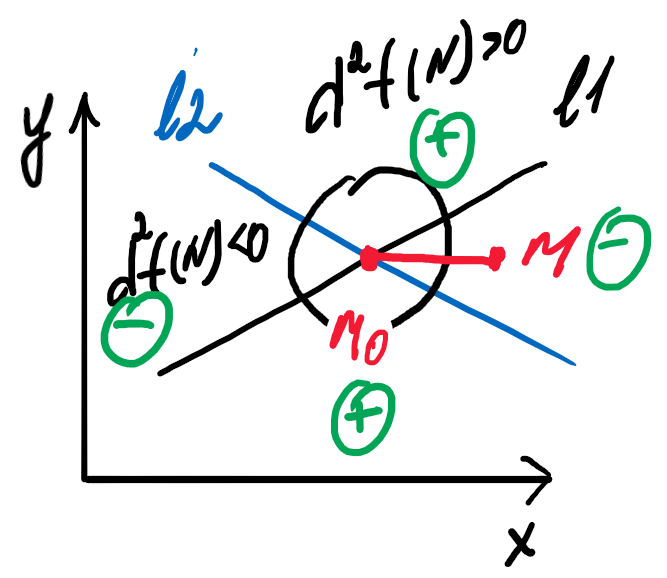
\includegraphics[width=35mm]{pictures/1_2_1.png}
                    \caption{}
                }
            \end{figure}
            \begin{align*}
                &l_1:\: (x - x_0) - \theta_1\,(y - y_0) = 0\\
                &l_2:\: (x - x_0) - \theta_2\,(y - y_0) = 0
            \end{align*}
            Таким образом мы видим
            \begin{align*}
                &\forall \varepsilon < \delta, \, \varepsilon > 0 \; & \exists M_1 \; d^2f(N_1) > 0 \; f(M) > f(M_1)\\
                & & \exists M_2 \; d^2f(N_2) > 0 \; f(M) < f(M_2)
            \end{align*}
        \end{enumerate}
    \end{Proof}

    \begin{Th}[Достаточное условие экстремума функции n - переменных]
        Пусть есть функция $u = f(M) = f(x_1, \dots, x_n) \in C^2(U(M_0))$ и $df(M_0) = 0$.\\
        Обозначим $d^2f(M_0) = \sum_{j = 1}^{n} \sum_{i = 1}^{n} a_{ij} dx_i dx_j, \, a_{ij} = a{ji}$\\
        Тогда
        \begin{enumerate}
            \item $d^2f(M_0) > 0 \Leftrightarrow \Delta_1 > 0, \dots, \Delta_n > 0 \Rightarrow M_0$ --- точка строгого минимума функции
            \item $d^2f(M_0) < 0 \Leftrightarrow \Delta_1 < 0, \dots, \Delta_2 > 0, \dots, (-1)^n\Delta_n \Rightarrow M_0$ --- точка строгого максимума функции
            \item $d^2f(M_0) \text{неопределённая форма} \Leftrightarrow \text{в} M_0$ --- нет экстремума функции
        \end{enumerate}
    \end{Th}
    \begin{Proof}
        Аналогино доказательству предыдущей теоремы, воспользуемся формулой Тейлора
        \[
            f(M) = f(M_0) + \frac{1}{1!} df(M_0) + \frac{1}{2!} d^2f(N), \, f(M) - f(M_0) = \frac{1}{2} d^2f(N)
        \]
        \begin{enumerate}
            \item \begin{align*}
                &\Delta_1(M_0) > 0, \dots, \Delta_n(M_0) > 0\\
                &\Rightarrow \text{ из критерия Сильвестра } \exists \delta>0 \; \forall N \in U_\delta(M_0)\\
                &\Rightarrow \; \Delta_1(N) > 0, \dots, \Delta_n(N) > 0\\
                &\Rightarrow \; d^2f(N) > 0\\
                &\Rightarrow \; f(M) > f(M_0), \; \forall M \in \mathring{U}_\delta(M_0) \Rightarrow M_0 \text{ --- точка минимума функции}
            \end{align*}
            \item Доказывается аналогично
            \item Принимаем без доказательств
        \end{enumerate}
    \end{Proof}

    \begin{Note}
        Если квадратичная форма равна нулю, то требуются дополнительные исследования. Например взятие производной  выше второй, рассмотрение точек в $\delta(M_0)$ окрестности 
    \end{Note}

    %\begin{Example}
    %    \textcolor{red}{!!!!!!!!!!}
    %\end{Example}

    %\begin{Example}
    %    \textcolor{red}{!!!!!!!!!!}
    %\end{Example}